\documentclass{article}
\usepackage[utf8]{inputenc}
\usepackage{polski}
\usepackage{graphicx}
\usepackage{fancyhdr}
\usepackage{lastpage}
\usepackage{listings}


\pagestyle{fancy}

\fancyhf{}

\fancyfoot[C]{\thepage\ / \pageref{LastPage}} % Ustawienie numeracji stron w stopce

\fancypagestyle{plain}{ % Nadpisanie stylu strony tytułowej
    \fancyhf{}
    \renewcommand{\headrulewidth}{0pt} % Usunięcie nagłówka
    \fancyfoot[C]{\thepage\ / \pageref{LastPage}}
}

\title{Specyfikacja implementacyjna projektu 1 w języku C}
\author{Miłosz Mertka i Sebastian Grosfeld}
\date{\today}

\begin{document}

\maketitle

\tableofcontents

\newpage

% Poniżej ustawiany jest nagłówek
\setlength{\headheight}{23pt}
\lhead{Miłosz Mertka\\Sebastian Grosfeld}
\rhead{Specyfikacja implementacyjna\\projektu 1 w języku C}

\section{Cel projektu}
Cel projektu został opisany w dokumencie \textbf{"Specyfikacja funkcjonalna\linebreak projektu 1 w języku C"} w pliku \emph{Specyfikacja\textunderscore funkcjonalna.pdf}.

\section{Algorytmy}
\subsection{Algorytm BFS}
Algorytm BFS nazywany jest algorytmem \emph{przeszukiwania grafu wszerz}.\linebreak W projekcie znajduje on zastosowanie przy sprawdzaniu, czy dany graf jest spójny. Zasada działania algorytmu BFS polega na odwiedzaniu kolejnych wierzchołków grafu do momentu aż nie pozostanie więcej wierzchołków do odwiedzenia. Jeżeli któreś wierzchołki nie zostały odwiedzone to oznacza, że graf jest niespójny. Algorytm korzysta z kolejki \textbf{FIFO} (\textbf{F}irst-\textbf{I}n-\textbf{F}irst-\textbf{O}ut), w celu przechowywania odwiedzonych wierzchołków.

\medskip

\noindent Algorytm BFS jako lista kroków:
\begin{enumerate}
    \item Dodaj wierzchołek 1 do kolejki.
    \item Dodaj do kolejki wszystkie nieodwiedzone wierzchołki połączone z wierzchołkiem, który jest pierwszy w kolejce.
    \item Usuń pierwszy wierzchołek z kolejki.
    \item Pobierz następny element z kolejki.
    \item Powtarzaj czynności od 2 do 4 dopóki wszystkie wierzchołki nie zostaną odwiedzone.
\end{enumerate}

\newpage

\subsection{Algorytm Dijkstry}
Algorytm Dijkstry służy do wyznaczania najkrótszych ścieżek od wierzchołka źródłowego do wszystkich innych wierzchołków grafu. Algorytm działa wyłącznie dla grafów ważonych, którego wagi są nieujemne. W projekcie narzucony został także dodatkowy wymóg spójności danego grafu, aby mieć pewność,\linebreak że algorytm Dijkstry znajdzie zadane ścieżki. Algorytm Dijkstry definiuje zbiór $Q$, który jest \textbf{kolejką} przechowującą wierzchołki, dla których nie obliczono jeszcze najkrótszych ścieżek. Na początku działania algorytmu zbiór $Q$ zawiera wszystkie wierzchołki grafu. Zdefiniowany jest także wektor $D$, który zawiera odległości od zadanego wierzchołka do wierzchołka $D[i]$. Na koniec działania algorytmu wektor ten zawiera wyznaczone odległości najkrótszych ścieżek. Dodatkowo można zdefiniować jeszcze wektor $P$ zawierający poprzedniki \linebreak dla odpowiednich wierzchołków. Dzięki temu możliwe jest odtworzenie ścieżek.

\medskip

\noindent Algorytm Dijkstry jako lista kroków:
\begin{enumerate}
    \item Pobierz ze zbioru $Q$ wierzchołek $v$ o najmniejszej wartości $D[v]$ i usuń go ze zbioru.
    \item Dla każdego następnika $w$ wierzchołka $v$ sprawdź, czy aktualne oszacowanie odległości do wierzchołka $w$ jest większe od oszacowania odległości \linebreak do wierzchołka $v$ plus waga krawędzi $(v, w)$.
    Jeżeli tak, to zaktualizuj oszacowanie $D[w]$ wartością prawej strony powyższej nierówności.
    \item Powtarzaj czynności od 1 do 2 dopóki zbiór $Q$ nie jest pusty.
\end{enumerate}

\newpage

\section{Budowa programu}
\subsection{Diagram podziału na moduły (\emph{Rysunek \ref{fig:modulo}})}
\begin{figure}[htp]
        \centering
        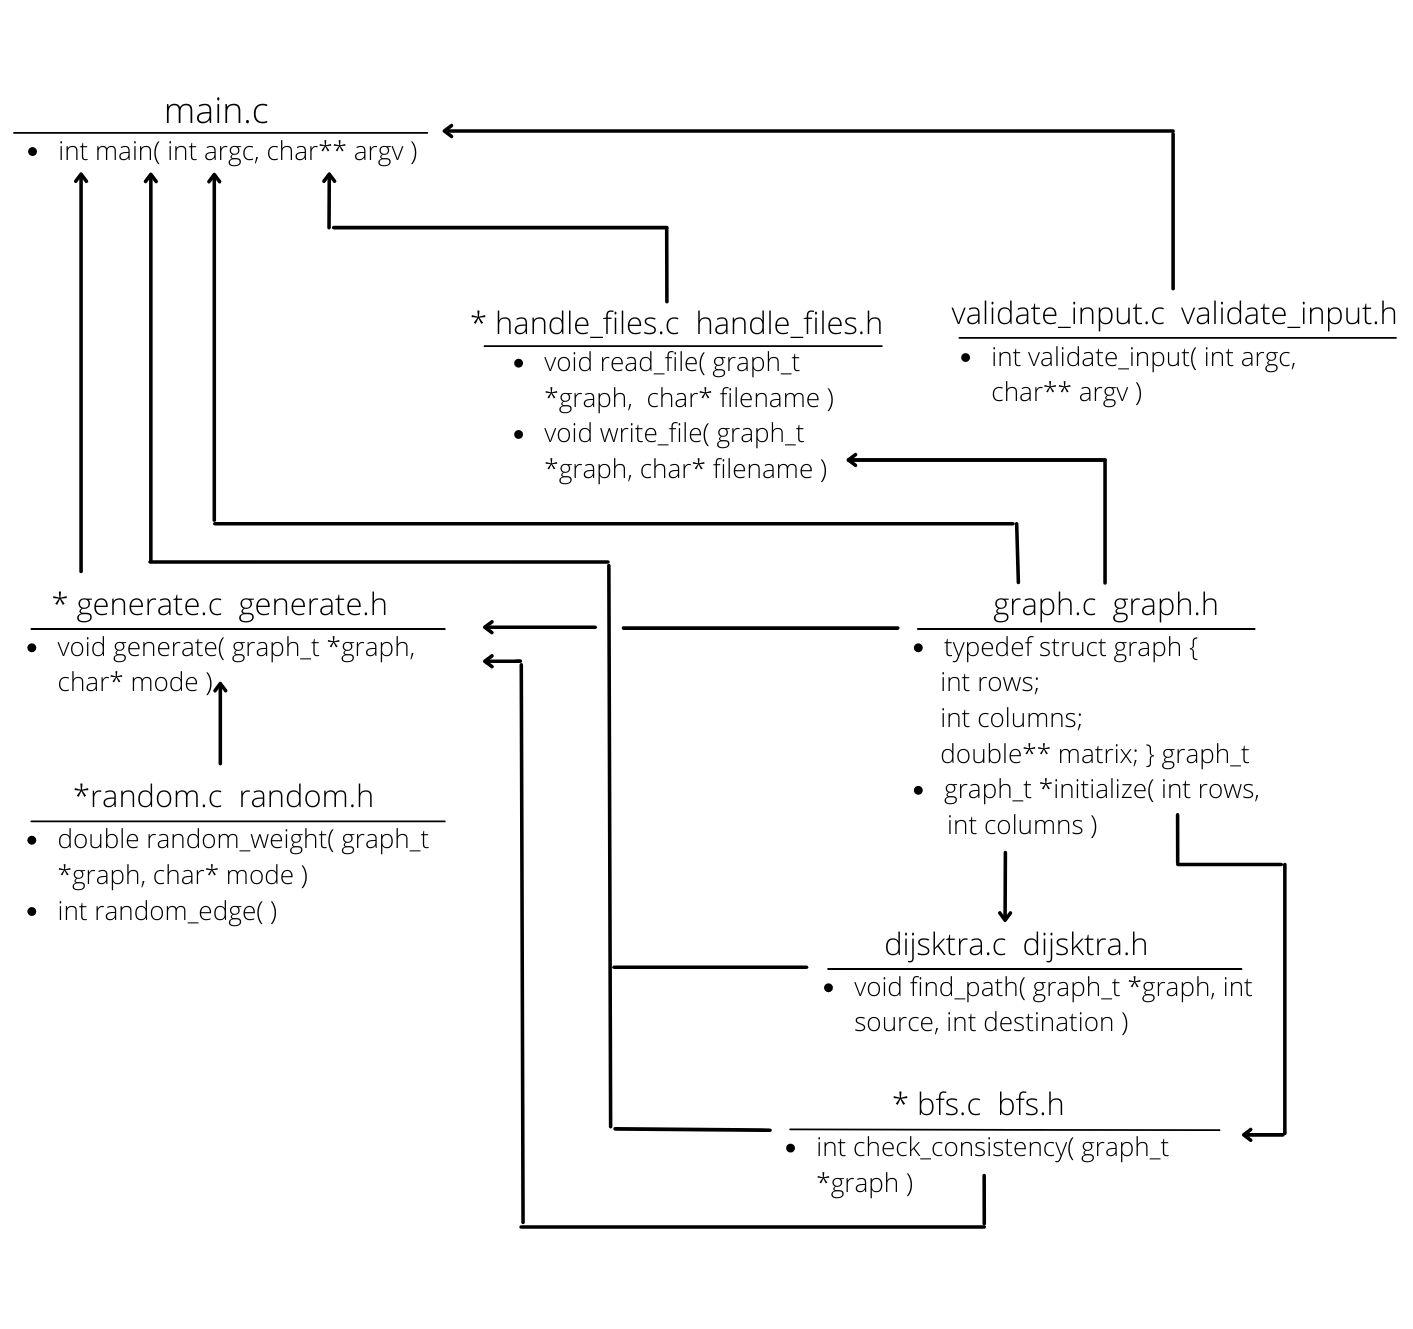
\includegraphics[width=14cm]{images/modulo.png}
        \caption{Podział programu na moduły}
        \label{fig:modulo}
\end{figure}

\newpage

\subsection{Opis stałych}
\begin{itemize}
    \item BOOL\textunderscore TRUE -- posiada wartość \textbf{1}. Stała jest stosowana jako oznaczenie wartości \emph{prawda}.
    \item BOOL\textunderscore FALSE -- posiada wartość \textbf{0}. Stała jest stosowana jako oznaczenie wartości \emph{fałsz}.
    \item GENERATE\textunderscore RANDOM\textunderscore MODE -- posiada wartość \textbf{"generate\textunderscore random"}. Jest to oznaczenie trybu działania programu \emph{generate\textunderscore random}.
    \item GENERATE\textunderscore CONSISTENT\textunderscore MODE -- posiada wartość \textbf{"generate\textunderscore consistent"}. Jest to oznaczenie trybu działania programu \emph{generate\textunderscore consistent}.
    \item GENERATE\textunderscore WAGES\textunderscore MODE -- posiada wartość \textbf{"generate\textunderscore wages"}. Jest to oznaczenie trybu działania programu \emph{generate\textunderscore wages}.
    \item ANALYZE\textunderscore MODE -- posiada wartość \textbf{"analyze"}. Jest to oznaczenie trybu działania programu \emph{analyze}.
\end{itemize}

\subsection{Opis struktur}
\begin{itemize}
    \item \textbf{graph} -- struktura opisuje graf i jest użyta do zdefiniowania typu \emph{graph\textunderscore t}.
    
    
    Posiada 3 pola:
    \begin{itemize}
        \item \textit{\textbf{int} rows} -- liczba wierszy grafu,
        \item \textit{\textbf{int} columns} -- liczba kolumn grafu,
        \item \textit{\textbf{int} **matrix} -- \textbf{macierz sąsiedztwa} służąca do zdefiniowania grafu w pamięci komputera. Indeksy wierszy i kolumn oznaczają wierzchołki, a komórki określają wartość wagi łączącej wierzchołki (oraz sam fakt istnienia krawędzi).
    \end{itemize}
\end{itemize}

\newpage

\subsection{Opis funkcji}
\begin{itemize}
    \item \textbf{int main(int argc, char **argv)} -- główna funkcja programu. Steruje jego działaniem.
    \begin{itemize}
        \item Wartość zwracana: kod wyjścia z programu.
        \item Argumenty:
            \begin{itemize}
                \item \textit{\textbf{int} argc} -- liczba argumentów przekazanych do programu w trakcie jego wywoływania,
                \item \textit{\textbf{char} **argv} -- lista argumentów przekazanych do programu \linebreak w trakcie jego wywoływania.
            \end{itemize}
    \end{itemize}
    
    \item \textbf{int validate\textunderscore input(int argc, char **argv)} -- funkcja walidująca poprawność przekazanych do programu argumentów.
    \begin{itemize}
        \item Wartość zwracana: \textbf{BOOL\textunderscore FALSE} jeśli dane są nieprawidłowe \linebreak lub \textbf{BOOL\textunderscore TRUE} jeśli nie znaleziono błędów.
        \item Argumenty:
            \begin{itemize}
                \item \textit{\textbf{int} argc} -- liczba argumentów przekazanych do programu w trakcie jego wywoływania,
                \item \textit{\textbf{char} **argv} -- lista argumentów przekazanych do programu \linebreak w trakcie jego wywoływania.
            \end{itemize}
    \end{itemize}
    
    \item \textbf{graph\textunderscore t *initialize(int rows, int columns)} -- inicjalizacja struktury przechowującej graf.
    \begin{itemize}
        \item Wartość zwracana: zainicjalizowana struktura grafu.
        \item Argumenty:
            \begin{itemize}
                \item \textit{\textbf{int} rows} -- liczba wierszy grafu,
                \item \textit{\textbf{int} columns} -- liczba kolumn grafu.
            \end{itemize}
    \end{itemize}
    
    \item \textbf{void generate(graph\textunderscore t *graph, char *mode)} -- generowanie grafu. Funkcja generuje graf na różne sposoby w zależności od trybu działania programu.
    \begin{itemize}
        \item Wartość zwracana: \textit{brak}.
        \item Argumenty:
            \begin{itemize}
                \item \textit{\textbf{graph\textunderscore t} *graph} -- struktura przechowująca graf,
                \item \textit{\textbf{char} *mode} -- tryb działania programu.
            \end{itemize}
    \end{itemize}
    
\newpage
    
    \item \textbf{double random\textunderscore weight(double min, double max)} -- losowanie wartości wagi dla krawędzi.
    \begin{itemize}
        \item Wartość zwracana: losowa liczba z zadanego przedziału.
        \item Argumenty:
            \begin{itemize}
                \item \textit{\textbf{double} min} -- minimalna wartość do wylosowania,
                \item \textit{\textbf{double} max} -- maksymalna wartość do wylosowania.
            \end{itemize}
    \end{itemize}
    
    \item \textbf{int random\textunderscore edge()} -- losowanie istnienia krawędzi między wierzchołkami.
    \begin{itemize}
        \item Wartość zwracana: \textbf{BOOL\textunderscore FALSE} jeśli krawędź nie istnieje \linebreak lub \textbf{BOOL\textunderscore TRUE} jeśli krawędź istnieje.
        \item Argumenty: \textit{brak}.
    \end{itemize}
    
    \item \textbf{void read\textunderscore file(graph\textunderscore t *graph, char *filename)} -- funkcja czytająca graf z pliku i zapisująca go do struktury.
    \begin{itemize}
        \item Wartość zwracana: \textit{brak}.
        \item Argumenty:
            \begin{itemize}
                \item \textit{\textbf{graph\textunderscore t} *graph} -- struktura przechowująca graf,
                \item \textit{\textbf{char} *filename} -- nazwa pliku definiującego graf.
            \end{itemize}
    \end{itemize}
    
    \item \textbf{void write\textunderscore file(graph\textunderscore t *graph, char *filename)} -- funkcja zapisująca graf do pliku.
    \begin{itemize}
        \item Wartość zwracana: \textit{brak}.
        \item Argumenty:
            \begin{itemize}
                \item \textit{\textbf{graph\textunderscore t} *graph} -- struktura przechowująca graf,
                \item \textit{\textbf{char} *filename} -- nazwa pliku wyjściowego.
            \end{itemize}
    \end{itemize}
    
    \item \textbf{int check\textunderscore consistency(graph\textunderscore t *graph)} -- sprawdzenie spójności zadanego grafu.
    \begin{itemize}
        \item Wartość zwracana: \textbf{BOOL\textunderscore FALSE} jeśli graf jest niespójny \linebreak lub \textbf{BOOL\textunderscore TRUE} jeśli graf jest spójny.
        \item Argumenty:
            \begin{itemize}
                \item \textit{\textbf{graph\textunderscore t} *graph} -- struktura przechowująca graf.
            \end{itemize}
    \end{itemize}
    
    \item \textbf{void find\textunderscore path(graph\textunderscore t *graph, int source, int destination)} -- szukanie najkrótszej ścieżki w grafie od zadanego wierzchołka źródłowego \linebreak do wierzchołka docelowego.
    \begin{itemize}
        \item Wartość zwracana: \textit{brak}.
        \item Argumenty:
            \begin{itemize}
                \item \textit{\textbf{graph\textunderscore t} *graph} -- struktura przechowująca graf,
                \item \textit{\textbf{int} source} -- numer wierzchołka źródłowego,
                \item \textit{\textbf{int} destination} -- numer wierzchołka docelowego.
            \end{itemize}
    \end{itemize}
\end{itemize}

\section{Środowisko programistyczne}
\begin{itemize}
    \item Język programowania: \textbf{C}
    \item Kompilator języka C: \textbf{GCC 7.3.0}
    \item System operacyjny: \textbf{Ubuntu 18.04 LTS}
    \item System kontroli wersji: \textbf{Git 2.17.2}
    \item Dodatkowe oprogramowanie: \textbf{GNU Make 4.1}
\end{itemize}

\section{Praca z repozytorium}
\begin{itemize}
    \item Projekt wykorzystuje system kontroli wersji \textbf{Git}.
    \item Każdy moduł będzie tworzony na osobnej gałęzi.
    \item Nazwy gałęzi odzwierciedlają nazwy modułów (np. moduł \emph{graph} jest tworzony na gałęzi o nazwie \emph{graph})
    \item Jeżeli pojawi się potrzeba utworzenia gałęźi, która nie jest związana \linebreak w sposób jednoznaczny z modułem, to taka czynność jest dozwolona \linebreak(w tym wypadku nazwa gałęzi jest dowolna).
    \item Po ukończeniu prac implementacyjnych nad danym modułem jego gałąź będzie łączona z gałęzią główną.
    \item Dopuszcza się jednak pojedyncze commity tworzone bezpośrednio na gałęzi głównej, jeśli zajdzie taka potrzeba.
    \item Komentarze, jakimi opatrywane są commity, są dowolne (nie ma narzuconej żadnej konwencji pisania komentarzy).
\end{itemize}

\section{Konwencje nazewnicze}
\begin{itemize}
    \item \textbf{Makrodefinicje i stałe} -- wielkie litery i wyrazy oddzielone znakiem "\textunderscore" (np. \emph{MAX\textunderscore BUFFER\textunderscore SIZE}).
    \item \textbf{Funkcje, struktury, zmienne i definicje typów} -- snake\textunderscore case \linebreak (np. \emph{generate\textunderscore random()}). Ponadto definicje typów są zakończone napisem "\textunderscore t".
\end{itemize}

\newpage

\section{Testy programu}
\subsection{Pliki testowe}
Testy programu będą przeprowadzane za pomacą programu \textbf{Make}. Pliki używane do testów zostaną umieszczone w podkatalogu \emph{test\textunderscore files} głównego programu.

\medskip

\noindent Pliki:
\begin{itemize}
    \item \emph{t\textunderscore graph.txt} (\emph{Rysunek \ref{fig:wagi}}) -- przechowuje graf o wymiarach \textbf{4 x 4} z wszystkimi krawędziami i wagami.
\begin{lstlisting}
7 4
	 1 :0.3  4 :0.2 
	 5 :0.2  2 :0.6  0 :0.4 
	 6 :0.8  3 :0.4  1 :0.6
	 7 :0.5  2 :0.8 
	 8 :0.9  0 :0.8  5 :0.9 
	 1 :0.5  9 :0.3  6 :0.4  4 :0.4 
	 10 :0.7  7 :0.7  2 :0.2  5 :0.3 
	 6 :0.9  3 :0.7  11 :0.7 
	 4 :0.7  12 :0.5  9 :0.2 
	 13 :0.8  5 :0.8  8 :0.4  10 :0.4 
	 14 :0.5  6 :0.5  9 :0.7  11 :0.3 
	 15 :0.3  10 :0.6  7 :0.8 
	 13 :0.5  8 :0.5 
	 9 :0.7  12 :0.7  14 :0.4 
	 10 :0.8  15 :0.2  13 :0.2 
	 11 :0.7  14 :0.4 
\end{lstlisting}
\begin{figure}[htp]
    \centering
    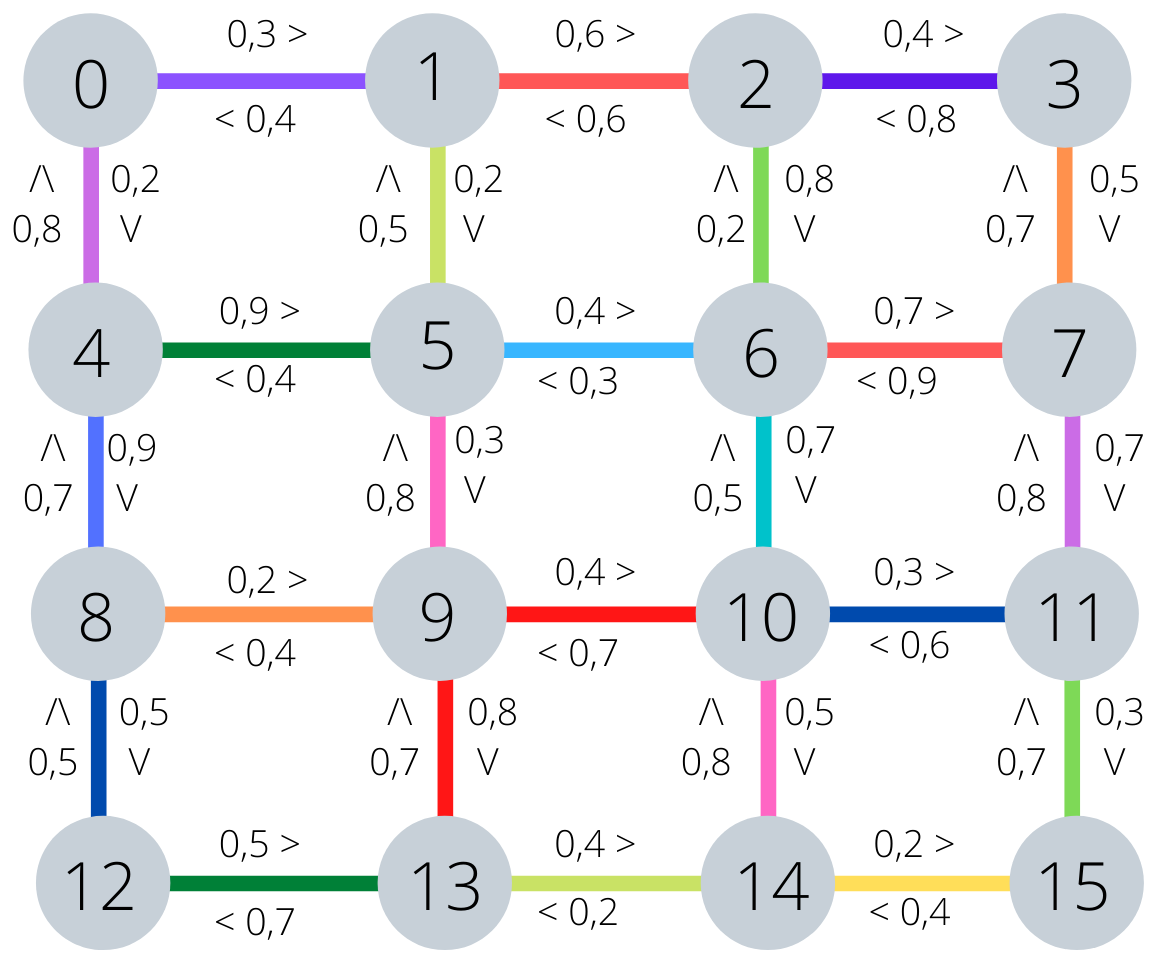
\includegraphics[width=7cm]{images/wagi.png}
    \caption{Wizualizacja pliku \emph{t\textunderscore graph.txt}}
    \label{fig:wagi}
\end{figure}
\item \emph{cos\textunderscore graph.txt} -- przechowuje graf spójny. Jest modyfikacją grafu z pliku \emph{t\textunderscore graph.txt}, w którym nie istnieje krawędź między wierzchołkami \textbf{15 i 11}.
\begin{lstlisting}
7 4
	 1 :0.3  4 :0.2 
	 5 :0.2  2 :0.6  0 :0.4 
	 6 :0.8  3 :0.4  1 :0.6
	 7 :0.5  2 :0.8 
	 8 :0.9  0 :0.8  5 :0.9 
	 1 :0.5  9 :0.3  6 :0.4  4 :0.4 
	 10 :0.7  7 :0.7  2 :0.2  5 :0.3 
	 6 :0.9  3 :0.7  11 :0.7 
	 4 :0.7  12 :0.5  9 :0.2 
	 13 :0.8  5 :0.8  8 :0.4  10 :0.4 
	 14 :0.5  6 :0.5  9 :0.7  11 :0.3 
	 10 :0.6  7 :0.8 
	 13 :0.5  8 :0.5 
	 9 :0.7  12 :0.7  14 :0.4 
	 10 :0.8  15 :0.2  13 :0.2 
	 14 :0.4 
\end{lstlisting}
\item \emph{incos\textunderscore graph.txt} -- przechowuje graf niespójny. Jest modyfikacją grafu z pliku \emph{t\textunderscore graph.txt}, w którym wierzchołek \textbf{11} nie jest połączony z żadnym innym wierzchołkiem.
\begin{lstlisting}
7 4
	 1 :0.3  4 :0.2 
	 5 :0.2  2 :0.6  0 :0.4 
	 6 :0.8  3 :0.4  1 :0.6
	 7 :0.5  2 :0.8 
	 8 :0.9  0 :0.8  5 :0.9 
	 1 :0.5  9 :0.3  6 :0.4  4 :0.4 
	 10 :0.7  7 :0.7  2 :0.2  5 :0.3 
	 6 :0.9  3 :0.7  
	 4 :0.7  12 :0.5  9 :0.2 
	 13 :0.8  5 :0.8  8 :0.4  10 :0.4 
	 14 :0.5  6 :0.5  9 :0.7   
	  
	 13 :0.5  8 :0.5 
	 9 :0.7  12 :0.7  14 :0.4 
	 10 :0.8  15 :0.2  13 :0.2 
	 14 :0.4 
\end{lstlisting}

\newpage

\item \emph{wf\textunderscore graph.txt} - przechowuje graf zapisany w nieprawidłowym formacie.
\begin{lstlisting}
7 4 1 :0.3  4 :0.2 
	1. 5 :0.2  2 :0.6  0 :0.4 
	2. 6 :0.8  3 :0.4  1 :0.6
	3. 7 :0.5  2 :0.8 
	4. 8 :0.9  0 :0.8  5 :0.9 
	5. 1 :0.5  9 :0.3  6 :0.4  4 :0.4 
	6. 10 :0.7  7 :0.7  2 :0.2  5 :0.3 
	 6 :0.9  3 :0.7  11 :0.7 
	 4 :0.7  12 :0.5  9 :0.2 
	 13 :0.8  5 :0.8  8 :0.4  10 :0.4 
	 14 :0.5  6 :0.5  9 :0.7  11 :0.3 
	 15 :0.3  10 :0.6  7 :0.8 
	 13 :0.5  8 :0.5 
	 9 :0.7  12 :0.7  14 :0.4 
	 10 :0.8  15 :0.2  13 :0.2 
	 11 :0.7  14 :0.4 
\end{lstlisting}
\end{itemize}

\subsection{Polecenia testujące}
\noindent Wywołania wraz z opisami:
\begin{itemize}
    \item \emph{make test\textunderscore file} -- wczyta graf zapisany w nieprawidłowym formacie z pliku \emph{wf\textunderscore graph.txt}.\\
    Oczekiwany rezultat:
    
    \medskip
    
    \emph{Invalid file format}
    \item \emph{make test\textunderscore arguments} -- wywoła program z nieprawidłowymi argumentami, a następnie z nieprawidłową liczbą argumentów.\\ Oczekiwany rezultat:
    
    \medskip
    
    \emph{Invalid mode}\\
    \emph{Invalid arguments}
    
    \item \emph{make test\textunderscore bfs} -- wczyta z pliku \emph{cos\textunderscore graph.txt} graf spójny i przeanalizuje go pod względem spójności. Następnie wczyta z pliku \emph{incos\textunderscore graph.txt} graf niespójny i powtórzy proces. Wypisze wyniki w konsoli.\\
    Oczekiwany rezultat:
    
    \medskip
    
    \emph{Consistent}\\
    \emph{Inconsistent}
    
\newpage
    
    \item \emph{make test\textunderscore dijsktra} -- wczyta graf z pliku \emph{t\textunderscore graph.txt} (\emph{Rysunek \ref{fig:wagi}}) i wypisze w konsoli informacje o wyniku testu. Program szuka najkrótszych ścieżek dla wierzchołków \textbf{0 i 3, 0 i 9, 10 i 2}.\\
    Oczekiwany rezultat:
    
    \medskip
    
    \emph{Test result: passed}
    \item \emph{make test\textunderscore graph} -- wygeneruje graf o wymiarach \textbf{7 x 4} ze wszystkimi krawędziami i wagami z przedziału \textbf{od 0 do 1} włącznie i zapisze go \linebreak do pliku \emph{test\textunderscore graph\textunderscore output.txt}.\\
    Oczekiwany rezultat:
    
    \medskip
    
    Program nie zgłosi żadnych błędów. Powstanie plik \emph{test\textunderscore graph\textunderscore output.txt} zawierający prawidłową definicję grafu.
    
\end{itemize}
\end{document}
